\chapter{Inledning}

För att drönare är mer versatila än robotar som inte flyger så finns det särskilda användningsfall för dem. De kan övervaka markföroreningar eller växternas behov av vatten och näring samt förhindra industriolyckor \citep{crowdsurveillance}. Drönare har också använts vid katastrofområden, som vid jordbävningen nära Japan för att mäta strålningsvärden i Fukushima och att skaffa visuell information om katastrofområdet samt i räddning av invandrare vid medelhavet. Inom logistikbranschen är man intresserad om autonoma drönaren som skulle leverera paket för kunder, till exempel 86 \% av Amazons paket väger mindre än 2.26 kg och de har tänkt på att leverera paket inom 30 minuter för människor som bor nära Amazons lager \citep{cbsnews}.

En drönare är ett obemannat luftfordon som kan styras med hjälp av visionsbaserad-, tröghets- eller satellitnavigation \citep{geospatial}. För att en drönare skulle kunna navigera självständigt måste den vara medveten om sitt läge, sin omgivning och sin hastighet. Andra faktorer som borde beaktas då en drönare flyger självständigt är hur drönare kan behandla data från inbyggda sensorer i sig, det vill säga kartlägga miljön och sin egen position i denna miljö samt hur man planerar vägen utan att kollidera med hinder.

Ett av de centrala forskningsfälten inom robotnavigering är navigering med hjälp av datorseende \citep{982903}. För att robotar skulle kunna navigera autonomt måste de kunna samtidigt kartlägga sin omgivning och lokalisera sig själv i omgivningen, som kallas för SLAM (Simultaneous Localization and Mapping). SLAM är ett problem som har fått uppmärksamhet av det vetenskapliga samfundet sedan 80-talet och har sätts som ett rön om det löses. Utmaningar i utvecklingen av kartläggnings- och lokaliseringsalgoritmer är att konstruera algoritmer som fungerar i allmänhet, som i dynamiska och stora miljön \citep{realslamproblem}. Sannolikhetsberäkning är tillvägagångssättet för att lösa SLAM-problemet och flesta av de algoritmer som har löst problemet baserar sig på sannolikhetsberäkning \citep{ProbabilisticRobotics}.

Avhandlingen är en översikt om SLAM-problemet och vilka metoder det finns för att kartlägga miljön och lokalisera sig själv med hjälp av datorseende. Frågor som behandlas är: Vad är det fundamentala problemet med SLAM-lösningarna? Vilka SLAM-metoder skulle kunna användas eller har använts med drönare och vad begränsar användningen av dessa? Varför har visionsbaserad navigation fått så mycket uppmärksamhet än andra navigeringsmetoder?

Resten av avhandlingen är strukturerad enligt följande: I kapitel 2 diskuteras bakgrund bakom visionsbaserad navigering. Vad är navigering och vilka sensorer kan användas i visionsbaserad navigering samt vilka metoder det finns för att extrahera data ur bilder. Kapitel 2 kommer också att diskutera lokalisering och kartläggning. Kapitel 3 är om samtidig lokalisering och kartläggning och hur SLAM kan grupperas i olika kategorier enligt hurudan data som man har. Kapitel 4 sammanfattar avhandlingen.

\chapter{Bakgrund}

\section{Visionsbaserad navigering}

Med navigering anser vi att en drönare planerar och utför en rutt från en given startplats till ett givet mål \citep{geospatial}. För att kunna navigera till målet måste drönaren vara medveten om sitt läge, sin miljö och sin hastighet. För att kunna navigera autonomt måste drönare kunna undvika hinder, planera sin rutt samt ta omvägar vid behov. I visionsbaserad navigering används visuella sensorer för att få bilder som indata. Bilderna behandlas sedan med algoritmer för att få en representation av omgivningen och för att lokalisera drönare i omgivningen. 

Visuella sensorer som används i visionsbaserad navigering är monokulära-, stereo-, RGB-D- och fisheye-kameror samt kombinationer av dessa \citep{geospatial}. En monokulärkamera innehåller ett kameraobjektiv och stereokamera har två kameraobjektiv. En fisheye-kamera är en monokulärkamera där man använder ett fisheye-objektiv för att få ett bredare synfält i bilden. Med RGB-D kamera kan man samtidigt ta bilder av omgivningen och uppskatta djuphet med hjälp av infrarödsensorer, oftast används dessa inomhus. 

Jämfört med de traditionella navigeringsmetoder, såsom satellitnavigering som använder GPS-signaler (Global Positioning System) för lokalisering, och tröghetsnavigering (Inerital Navigation System) som använder accelerometer och gyroskop, är fördelarna med kameror att man får visuell information, som till exempel färg, textur och former av omgivningen, det går att navigera i områden där GPS-signaler inte fungerar för att kameror är passiva, det vill säga de kan inte bli störda av utomstående signaler eller upptäckas av utomstående entitet. Med egenskapen att kameror är passiva kan man beräkna drönarens position i omgivningen inombords, dessutom är kamerasensorer billiga att operera och väger lite \citep{opticalflowuav,geospatial}.

Drönare byggs mindre än förr och har därför begränsad batteri- och bärkapacitet. Visionsbaserad navigering med drönare som använder sig av laser- och ultraljudsensorer har uteslutnas på grund av att dessa sensorer förbrukar mer elektricitet och väger mer än kameror \citep{6385934}. Med hjälp av visionsbaserad navigering som använder sig av kameror kan man få rikligt med information av omgivningen \citep{geospatial}. Visionsbaserad navigering, som är ett aktivt forskningsområde, är en av de mest lovande navigeringsmetod för robotnavigering.

\section{Bildbearbetning}

Med kameror får man sekventiella bilder ur omgivningen som sedan bearbetas med algoritmer för att få en representation av miljön \citep{982903}. Bildbearbetning betyder att man gör utdrag ur bilder i form av former, kanter, linjer, rörelse, färg eller mönster och bygger en karta av de egenskaper som man extraherat ur bilderna. 

För att extrahera landmärken ur bilder, det vill säga former, kanter eller linjer, så finns det olika bilbearbetningsalgoritmer såsom SIFT (Scale-Invariant Feature Transform), HARRIS hörnupptäckare, SURF (Speeded Up Robust Features), ORB (Oriented FAST and Rotated BRIEF), med mera \citep{orb, slamproblem, mapbuildingsift}. SIFT, SURF och ORB prövar hitta egenskaper från bilderna som är invarianta för rotation, som menar att samma egenskaper kan hittas från olik synvinkel \citep{orb}. 

Algoritmerna fungerar i allmänhet så att de går igenom bilderna per pixelnivå där de provar hitta områden i bilderna som har stora skillnader i färgnyanser. Till exempel ORB-bildbearbetningsalgoritmen är en kombination av flera algoritmer som söker egenskaper ur bilder och konstruerar landmärken av dessa egenskaper, som sedan kan sparas för senare användning. 
Till början så använder ORB en algoritm som söker skillnader i ljusstyrka runtomkring varje pixel och om det finns en stor skillnad på färgnyansen i pixlarna runtomkring så använder den området som en egenskap i bilden. Efter att algoritmen har hittat egenskaperna så används HARRIS-hörnupptäckningsalgoritmen för att filtrera bort egenskaper som inte upptäcks av HARRIS, då har man kvar egenskaper ur bilden som är invariant för rotation \citep{orb}. 

För de egenskaper som är kvar efter filtreringen används det algoritmer för att avbilda hur de egenskaperna skulle se ut då man roterar eller skalar bilden, och med hjälp av dessa algoritmer går det att spara egenskaperna som landmärken i kartan, och senare förena observerade landmärken från olik synvinkel och avstånd, till de som man har i kartan \citep{orb}. Enligt \cite{orb} är ORB mer energieffektiv bildbearbetningsalgoritm än SIFT för att den kräver mindre beräkning för att extrahera egenskaper och konstruera landmärken ur bilder, som betyder att den är snabbare färdig, utan att tappa effektivitet för att hitta landmärken.

Då man extraherar egenskaper ur bilder är det möjligt att utjämna bilder \citep{mapbuildingsift}. Detta menar att man gör bilder otydligare för att få bort digitalt brus och att bilden har mindre detalj. Då man extraherar egenskaper ur bilder som är otydligare hittar algoritmerna färre egenskaper än om bilden var i sin originalform. Med att extrahera färre egenskaper ur bilderna då en robot navigerar kan algoritmerna beräkna snabbare robotens läge i omgivningen, på grund av att beräkningstiden är mindre för att matcha alla landmärken man observerat med tidigare observationerna.

Fast det finns fördelar på detalj av omgivningen man får då man använder kameror, så jämfört med andra sensorer, som till exempel laser och ultraljud, är förändring i belysning, vädret och årstid samt skuggor ett problem som måste tas i beaktande med kameror, speciellt då man navigerar utomhus \citep{982903}. Dessa problem har lösts med att bearbeta bildernas färgnyanser, färgmättnad (saturation) och ljusstyrka.

\section{Lokalisering i omgivningen}

Med att en robot lokaliserar sig själv menar vi att den tar reda på sin position i omgivningen \citep{982903}. Från bilderna ur kameror i drönaren identifieras landmärken, sedan matchas de observerade landmärken med de som finns i kartan och efter det kan drönaren estimera sin position i omgivningen. Lokalisering av en drönare är enkelt då man har en uppfattning om miljön, till exempel en karta.

Då en drönare navigerar så beräknas positionen och orientationen av drönaren till exempel med sannolikhetsberäkning baserat på tid och indata av sensorer \citep{ProbabilisticRobotics}. Efter varje rörelse drönaren gör måste den estimera sin position i omgivningen. För att beräkna sannolikheten av sin position i omgivningen använder den som data rörelseinformation, och efter att den har rört på sig, observerade landmärken. Med att drönare observerar landmärken efter sin rörelse kan den förstärka sin sannolikhet om sin position i omgivningen. 

Då man använder sannolikhetsberäkning för lokalisering är robotens läge i omgivningen en kontinuerlig stokastisk sanningsvariabel $X$, där en sannolikheten av robotens läge betecknas som $P(x_t)$, alltså möjligheten att roboten befinner sig vid $x$ vid tidpunkt $t$, som är samma sak som att $P(X = x_t)$ \citep{ProbabilisticRobotics}. Variabeln $x_t$ beskriver då robotens tillstånd, som i drönarens fall kan vara till exempel drönarens koordinater och orientering i omgivningen. Rörelseinformation som skaffas vid tidpunkt $t$ betecknas som $u_t$ och landmärken som extraheras från kamerasensorernas bilder med $z_t$. Lokaliseringsproblemet är att bestämma $x_t$ med sannolikhetsberäkning givet alla föregående lägen $x_{0:t-1}$, landmärkesuppfattningar $z_{1:t-1}$ och rörelseinformationer $u_{1:t}$ samt då vi antar att roboten rör på sig före den skaffar sensorinformationen. Då kan betingade sannolikhetsformeln för robotens läge vid $X = x_t$ skrivas som:
\begin{align}
    P( X = x_t | x_{0:t-1}, z_{1:t-1}, u_{1:t})
\end{align}

Problem uppstår i beräkningen då man navigerar länge för att man tar i beaktande alla tidigare lägen $x_{0:t-1}$ för att beräkna nästa läge \citep{ProbabilisticRobotics}. För att minska beräkningsbehov i lokaliseringsproblemet antar man Markovegenskapen för variabeln $x$. Med Markovegenskapen menar man att läge vid $x_t$ är bara beroende på den tidigare läge, alltså sannolikheten $x_{t-1}$, och inte på händelseförloppet som hände före roboten befinner sig vid $x_{t-1}$. Då man antar att $x$ har Markovegenskapen så kan man begränsa att $x_t$ är bara beroende på den tidigare position $x_{t-1}$ och rörelseinformation $u_t$, se figur \ref{markov}, som demonstrerar Markovegenskapen. Lokaliseringsproblemet kan då skrivas som följande:
\begin{align}
    P(x_t | x_{t-1}, u_{t})
\end{align}

Då vi antar att roboten rör på sig och sedan skaffar sensorinformation och att $x_t$ har Markovegenskapen kan sannolikhetsfördelningen för landmärkesuppfattningar $z_t$ skrivas:

\begin{align}
    P(z_t | x_{0:t}, z_{1:t-1}, u_{1:t}) = P(z_t|x_t)
\end{align}

Formeln $P(x_t|x_{t-1}, u_{t})$ är rörelseuppfattningssannolikheten och $P(z_t|x_t)$ är landmärkesuppfattningssannolikheten för roboten \citep{ProbabilisticRobotics}. 

\begin{figure}[ht]
    %\begin{figure}[tbh] t= top, b = bottom, h=here
    \begin{center}
    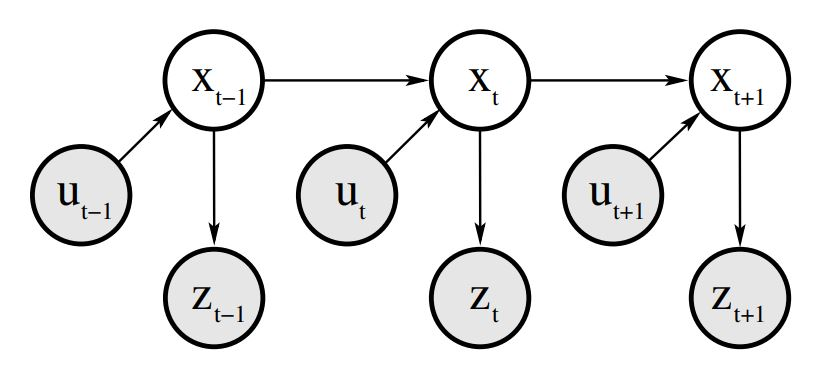
\includegraphics[width=0.75\textwidth]{markov.JPG}
    \caption{Lokaliseringsproblemet med Markovegenskapen är att bestämma $x_t$ givet $x_{t-1}$ och $u_t$. En bild på lokaliseringsproblemet som visualiserar Markovegenskapen för variabeln $x$ \citep{ProbabilisticRobotics}.}
    \label{markov}
    \end{center}
\end{figure}

Läget av roboten kan beräknas med Bayes filter som använder sig av rörelse- och landmärkesuppfattningssannolikheten \citep{ProbabilisticRobotics}. Bayes filter är en rekursiv algoritm som beräknar sannolikheten för robotens position baserat på robotens tidigare position, rörelseinformation och observerade landmärken. I Bayes filter algoritmen beräknas $bel(x_t)$, som är en sannolikhetsfördelning av robotens position i omgivningen.

\begin{algorithm}[H]
    \SetAlgoLined
    \SetAlgoRefName{BFA}
    \label{BFA}
    \FuncSty{BayesFilter($bel(x_{t-1})$, $u_t$, $z_t$):} \\
    \ForAll{$x_t$}{
        $spådom$ = $\int P(x_t | x_{t-1}, u_t) bel(x_{t-1}) dx_{t-1}$ \\
        $bel(x_t)$ = $\eta P(z_t | x_t)$ $spådom$
    }
    \Return{$bel(x_t)$}
    \caption{Bayes Filter Algoritm}
\end{algorithm}

Bayes filters algoritmen fungerar så att för varje $x_t$ beräknas två kritiska steg, som är spådom och korrigering \citep{ProbabilisticRobotics}. Spådomsdelen i algoritmen är delen där vi beräknar integralen för två faktorer: sannolikheten att rörelseinformationen $u_t$ tar oss till $x_t$ och den gamla distributionen av positionen $bel(x_{t-1})$. Korrigeringsdelen är då man multiplicerar spådomsdelen med den sannolikhet att $z_t$ skulle observeras för varje möjliga $x_t$. I korrideringsdelen används en normering konstant $\eta$ för att normera sannolikheten. Bayes filter algoritmen är definierat nedan som sedan görs rekursivt, se algoritmen \ref{BFA}. Utmaningen i algoritmen är integralen i spådomsdelen. För att algoritmen skulle fungera i allmänhet, måste man begränsa robotens läge att vara en ändlig variabel så att integralen över spådomsdelen blir en summa. 

Med hjälp av Bayes regler, lagen om total sannolikhet för kontinuerliga variabler och Markovegenskapen kan det bevisas med matematisk induktion att Bayes filtern fungerar, då man antar att $x_t$ har Markovegenskapen och att $bel(x_0)$ sannolikhetsfördelning är känd då $t = 0$. Med att sannolikhetsfunktionen är känd menar vi att roboten vet sin position vid början med full säkerhet eller så är $bel(x_0)$ en likformig sannolikhetsfördelning.

\begin{align}
bel(x_t) & = P(x_t | z_{1:t}, u_{1:t}) \tag{BF1}\label{BF1} \\
        & = \eta P(z_t | x_t, z_{1:t-1}, u_{1:t}) P(x_t | z_{1:t-1}, u_{1:t}) \tag{BF2}\label{BF2}\\
        & = \eta \underline{P(z_t | x_t)} P(x_t | z_{1:t-1}, u_{1:t}) \tag{BF3}\label{BF3}\\
        & = \eta P(z_t | x_t) \underline{\int P(x_t | x_{t-1}, z_{1:t-1}, u_{1:t}) P(x_{t-1} | z_{1:t-1}, u_{1:t}) dx_{t-1}} \tag{BF4}\label{BF4}\\
        & = \eta P(z_t | x_t) \int \underline{P(x_t | x_{t-1}, u_t)} P(x_{t-1} | z_{1:t-1}, u_{1:t}) dx_{t-1} \tag{BF5}\label{BF5}\\
        & = \eta P(z_t | x_t) \int P(x_t | x_{t-1}, u_t) P(x_{t-1} | z_{1:t-1}, \underline{u_{1:t-1}}) dx_{t-1} \tag{BF6}\label{BF6}\\
        & = \eta P(z_t | x_t) \int P(x_t | x_{t-1}, u_t) \underline{bel(x_{t-1})} dx_{t-1} \tag{BF7}\label{BF7}
\end{align}

Sannolikhetsfördelningen i Bayes filter är \ref{BF1}, det vill säga sannolikheten att roboten är vid $x_t$, som betecknas $bel(x_t)$, är samma som sannolikheten av $x_t$ givet $z_{1:t}$ och $u_{1:t}$. Med Bayes teorem kan detta skrivas om i format \ref{BF2}. Vid \ref{BF3} använder vi Markovegenskapen för $x_t$ så kan betingade sannolikheten för $z_t$ skrivas som landmärkesuppfattningssannolikheten. Med satsen om total sannolikhet för kontinuerliga variabler, som uttrycker sannolikheten för enskilda händelser till en betingade sannolikhet, kan formeln skrivas om till \ref{BF4}. Vid \ref{BF5} och \ref{BF6} använder vi Markovegenskapen för $x_t$, se Markovkedjan i figur \ref{markov}. Till slut får vi \ref{BF7}, som bevisar med induktion att algoritmen fungerar \citep{ProbabilisticRobotics}.

Bayes filter är den mest allmänna algoritm för att beräkna robotens läge med sannolikhetsberäkning \citep{ProbabilisticRobotics}. Algoritmen baserar sig starkt på Markovegenskapen att det nuvarande läge är oberoende av tidigare data. I robotnavigering är det inte dock så lätt att anta detta, för det skulle betyda att allt runtomkring roboten borde vara statiskt. Till exempel om en bil rör på sig då roboten navigerar så då man gör landmärkesuppfattning kommer Bayes filter algoritmen att ge en felaktig estimation. Bayes filter är basis för många andra lokaliseringsalgoritmer, som till exempel Kalman filter eller Markov lokalisation. 

I navigering är det svårt att begränsa robotens tillstånd så att integralen i Bayes filter blir en summa över spådomsdelen, för det skulle betyda att roboten navigerar i en begränsad omgivning. På grund av oändligt läge där roboten kan befinna sig i omgivningen beräknar lokaliseringsalgoritmer ett approximativt värde för sannolikhetsfördelningen och det är i beräkningen av approximativa värdet där olika lokaliseringsalgoritmer skiljer sig \citep{ProbabilisticRobotics}.

Med att approximera sannolikhetsfördelningen så lämnar man bort någon av egenskaperna som är viktigt för robotnavigering, såsom beräkningseffektivitet, noggrannhet i approximerande av robotens läge eller enkel implementering av algoritmen för robotar, för att förbättra någon annan av egenskaperna \citep{ProbabilisticRobotics}. Till exempel om man vill nå beräkningseffektivitet då man approximerar så avstår man till exempel i noggrannhet av robotens läge.

Lokalisering kan delas i global och lokal lokalisering \citep{982903, globalsubmaps}. Med global lokalisering har roboten ingen vetskap om sin position vid början av navigeringen. I lokal lokalisering har roboten en ungefärlig eller exakt vetskap om sin plats vid början av navigeringen som den fått som indata. 

Lokala lokaliseringsmetoder strävar för att korrigera fel som uppstår av robotens rörelse. Med globala lokaliseringsmetoder kan roboten klara av verkliga misstag då den estimerar sin position i omgivningen, till exempel roboten kan klara av en situation där den kidnappas och förs till en annan plats. Då man börjar navigera, alltså när tidpunkt $t$ är noll, så då man använder sig av globala lokaliseringsmetoder är sannolikheten att roboten är vid $bel(x_0) = 1 / |X|$ och i lokala lokaliseringsmetoder är det till exempel $bel(x_0) = 1$ eller en normalfördelning runt läget $x_0$ \citep{ProbabilisticRobotics}.

\section{Kartläggning av omgivningen} \label{kartlaggning}

Med kartläggning av omgivningen menar vi att roboten kartlägger sin omgivning med hjälp av data som den har tillgång till, detta kan vara till exempel rörelseinformation eller sensorinformation samt kombinationer av dessa \citep{ProbabilisticRobotics}. I lokal lokalisering, där man vet robotens läge och har åtkomst till rörelseinformation, är kartläggning lättare att göra än då robotens position i början är okänd. För att konstruera en karta så måste man ta i beaktande störningar som uppstår av rörelse- och sensorinformation.

En karta om miljön kan representeras i två (2D) eller tre (3D) dimensioner \citep{geospatial}. Att konstruera en 3D-representation av omgivningen kräver det mer beräkningskapacitet än att konstruera en 2D-karta, för att man tar i beaktande fler dimensioner \citep{ProbabilisticRobotics}. För robotar som navigerar på stadig grund är oftast en 2D-representation tillräckligt, men för drönaren behöver man kartlägga i 3D. 

För att konstruera 3D-kartor behöver man uppskatta djuphet. Metoder för att uppskatta djuphet med datorseende är till exempel att beräkna binokulära skillnaden eller rörelseparallax \citep{suomimainittu}. Idén med att beräkna binokulära skillnaden och rörelseparallax är att uppskatta djuphet på samma sätt som mänskliga synförmåga.

Rörelseparallax betyder att objekt rör på sig snabbare i synfältet då de är närmare observatören och långsammare då de är långt borta, detta gäller också om observatören rör på sig och objektet står stilla \citep{suomimainittu, parallax}. För att räkna binokulära skillnaden för observerade kännetecken behöver man två kameror som är riktade parallellt i samma linje så att deras synfält överlappar, kamerornas distans från varandra är känd och av båda kamerornas bilder utdras samma kännetecken. Från skillnaden ur kännetecknets horisontala position i båda av kamerornas bilder kan man estimera djuphet. Med en monokulär kamera kan man uppskatta djuphet av bilder baserat på rörelseparallax. För att estimera djuphet med monokulärkamera och rörelseparallax behöver man veta distansen till ett objekt då navigeringen börjar och som indata får man bilder och rörelseinformation av roboten. Rörelseinformationen i robotar på stadig grund kan man få till exempel från en hastighetsmätare som är inbyggt i roboten.

\cite{suomimainittu} undersökte djuphetsuppskattning med rörelseparallax och med att räkna binokulära skillnaden från stereokameror, och märkte att stereokameror fungerar bättre då objekten är nära medan monokulära kameror med hjälp av rörelseparallax kan uppfatta mer precis distans då distansen växer \citep{suomimainittu}. Med stereokamera kan djupheten estimeras bra upp till cirka 10 meters avstånd och vid 20 meters avstånd så är estimeringarna oanvändbara, efter detta måste man växla över till att använda monokulära kameran. \cite{suomimainittu} skriver att forskning för att skaffa rörelseinformation från bilderna är viktigt, på grund av att rörelseinformation behövs för att lokalisera roboten i omgivningen och kartlägga omgivningen. Med att uppskatta rörelseinformation från bilder kan man avlägsna hastighetsmätare som drönare inte har tillgång till och detta ger möjlighet att estimera djuphet ur bilderna för drönare.

Kartor kan sparas i olika format, såsom datorstödd konstruktion (CAD, Computer-Aided Design), beläggningskarta (Occupancy Grid Map) eller en enkel graf om landmärken och deras sammankopplingar \citep{982903}. En datorstödd konstruktion av miljön kan vara en mycket detaljerad representation av omgivningen. En beläggningskarta är en 2D eller 3D-modell av omgivningen som är sparat i ett rutsystem där rutor som är upptagna är någon objekt i miljön, oftast har dessa rutorna sparat i sig en sannolikhet att där finns någon objekt i vägen \citep{6095058, 982903}. 

Kartan kan vara färdigt sparad för en drönare eller så kan miljön kartläggas från bilderna av sensorerna då den flyger \citep{geospatial}. Med 3D volymetriska sensorer kan man konstruera en 3D modell och spara denna information i en Octree-struktur. Med strukturen kan data om miljön packas i mindre format utan att tappa möjligheten att uppdatera informationen vid behov. En annan metod som tas upp är med stereovisionsalgoritmer göra en djuphetskarta och behandla data till plana ytor som minskar på missvisning som uppstår med användning av stereovision algoritmer när man bygger upp djuphetskartan. 

Viktigt i kartläggning är att kartan kan lätt uppdateras då man gör nya observationer och bevarar data om hur landmärken är sammankopplade, för att då man observerar nya landmärken och får beräknat en bättre sannolikhet av robotens läge så uppdateras också landmärkes sannolikhet att de är vid positionen som man observerade \citep{globalsubmaps}.

Oftast så har robotar inte en färdig karta som de kan använda för att planera sin rutt eller att navigera, och för att åstadkomma autonoma robotar så måste de kunna själv kartlägga sin omgivning \citep{ProbabilisticRobotics}. Kartläggning för robotar är ett problem som är svårt utan lokalisering och lokaliseringsproblemet är svårt att lösa utan att man kartlägger, därför är det nyttigt att lösa båda problem samtidigt. 

\chapter{Samtidig lokalisering och kartläggning}

Samtidig lokalisering och kartläggning (SLAM) är ett av de grundläggande problem i robotnavigering \citep{realslamproblem}. SLAM-problemet definieras så att en robot som inte har tidigare information om sin plats eller omgivning skall samtidigt bygga en karta av omgivningen och lokaliserar sig själv relativt till kartan som den bygger, till exempel med hjälp av datorseende och att identifiera landmärken. Att beräkna robotens läge med sannolikhetsberäkning så är termen $P(x_t, m|z_{1:t}, u_{1:t})$, det vill säga, sannolikheten att roboten befinner sig vid $x_t$ och kartan $m$ givet alla landmärkesuppfattningar $z_{1:t}$ och rörelseinformation $u_{1:t}$. 

Det finns två varianter av SLAM-problemet, som är Fullständig SLAM och Online SLAM \citep{ProbabilisticRobotics}. Skillnaden med dessa två är hur man beräknar betingade sannolikheten för $x_t$ och $m$. I fullständig SLAM beräknas betingade sannolikheten från hela robotens positionskedja $x_{0:t}$, det vill säga $P(x_{0:t}, m | z_{1:t}, u_{1:t})$, medan i Online SLAM använder man bara senaste läge $x_{t-1}$ och kartan $m$, då är formeln $P(x_t, m | z_{1:t}, u_{1:t})$, alltså man döljer tidigare rörelse- och landmärkesinformation för att estimera den nya positionen av roboten. Några lösningar för SLAM som baserar sig på sannolikhetsberäkning är Extended Kalman Filter (EKF-SLAM), som är en Online SLAM-lösning, och FastSLAM, som är en fullständig SLAM-lösning \citep{realslamproblem, ProbabilisticRobotics}. 

\begin{figure}[ht]
    %\begin{figure}[tbh] t= top, b = bottom, h=here
    \begin{center}
    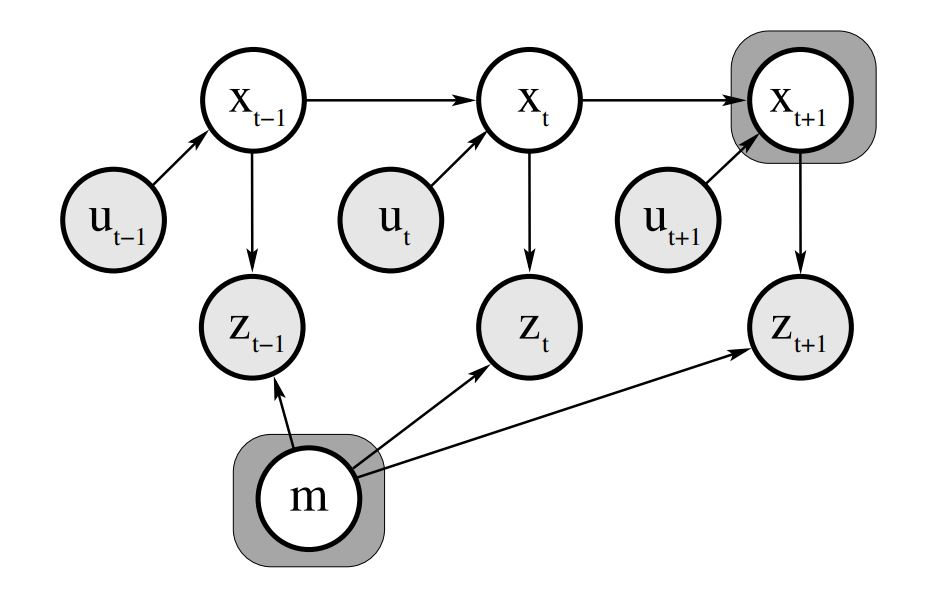
\includegraphics[width=0.8\textwidth]{online-slam.JPG}
    \caption{Bild på Online SLAM-problemet där man beräknar sannolikheten av robotens position och bygger kartan från sensorinformation $z$ och rörelseinformation $u$ \citep{ProbabilisticRobotics}.}
    \label{slam-problemet}
    \end{center}
\end{figure}

SLAM-problemet har delproblem som borde lösas för att få robotar att navigera autonomiskt \citep{slamproblem}. Ett stort problem i flesta visionsbaserade SLAM-lösningar är dataföreningsproblemet, som betyder att man identifierar två olika landmärken som en och samma. Detta problem kan uppstå redan vid korta rörelsen av robotar eller då en robot har navigerat och kommer till en plats som den har redan varit i förr, detta kallas för loopstängning (Loop Closure). Med att förena landmärken fel så uppkommer det missvisningar då man estimerar positionen av roboten.

Positionen av roboten i omgivningen och landmärkens position i kartan kan beräknas också med att räkna distansen till landmärken och bevara en matris om landmärkens sannolikhetsposition i omgivningen och landmärkes förhållande till varandra, alltså en korrelationsmatris \citep{realslamproblem, ProbabilisticRobotics}. Då man bevarar en korrelationsmatris så har man den fördelen att när man lokaliserar en robot med stor sannolikhet går det att uppdatera landmärkens sannolikhet av deras position. Nackdelen med denna metod är att då man observerat stora mängder av landmärken så kommer beräkningsbehovet att växa kvadratiskt enligt observerade landmärken. 

Visuell kartläggning och lokalisering kan delas i tre kategorier baserat på data som man har i början av navigeringen. Kategorierna är kartlösa (mapless), kartbaserade (map-based) och kartbyggande (map-building) system \citep{geospatial}. 

\section{Kartlösa system}

Kartlösa system är oftast den realistiska situationen då man navigerar \citep{ProbabilisticRobotics}. I system utan karta navigerar drönare bara med hjälp av att observera tydliga egenskaper i miljön \citep{982903}. Dessa kan vara till exempel väggar, dörrar, möbler eller andra landmärken. Metoder, som diskuteras i avhandlingen, och används inom kartlösa system är optiskt flöde (Optical flow) och spårning av egenskaper (Feature tracking). 

\subsection{Optiskt flöde}

Optiskt flöde hänvisar till uppfattad relativ rörelse i sekventiella bilder mellan observatören och till exempel någon fästpunkt i miljön \citep{opticalflowuav}. Rörelse uppstår i sekventiella bilder till exempel då man vänder kameran eller om något rör på sig då kameran är stilla. Från relativa rörelsen i sekventiella bilder kan man beräkna flödesvektorer.

För att demonstrera ett exempel hur optiskt flöde kan användas för robotnavigering har \cite{341094} använt optiskt flöde i en robot för att imitera bin \citep{341094}. De placerade två kameror, som är parallelt riktade ifrån varandra, på varsin sida av en robot och beräknade flödesvektorer från bilderna av båda kamerorna då roboten rör på sig. Om flödesvektorernas beräknade längd var samma på båda sidorna så far roboten rakt framåt, annars om andra sidas flödesvektoren är kortare än den andra så vänder den mot den sida vilkens flödesvektor är kortare. Med att använda optiskt flöde för navigering behöver man inte uppskatta djuphet. Denna navigeringsmetod fungerar dåligt i strukturlösa miljö där det inte finns någon fästpunkt eller landmärke som kan användas för att beräkna flödesvektorerna. 

Fastän metoden som \cite{341094} använde tog bara i beaktande horisontala flödesvektorer och demonstrerade att optiskt flöde kan användas i robotnavigering på stadig grund, så har sedan detta användning av optiska flödesmetoder använts i drönare \citep{6564752}. Nuförtiden används optiskt flöde i drönare för att uppskatta avstånd, hålla sin höjd, undvika hinder, beräkna hastighet och landa på en plattform som rör på sig.

\subsection{Spårning av egenskaper}

Spårning av egenskaper (Feature tracking) används för att skaffa information om objekt, såsom linjer, hörn och olika landmärken som är invariant för rörelse med hjälp av kameror och bildbearbetningsalgoritmer \citep{geospatial}. Med hjälp av dessa landmärken och deras relativa rörelse i sekventiella bilder kan man bestämma robotens position och bygga en karta. Då drönare navigerar i omgivningen, så kommer den troligtvis att se samma landmärken från olika perspektiv, som hjälper drönare att beräkna en bättre sannolikhet för sin position i omgivningen samt uppdatera landmärkes position i kartan. Traditionella SLAM-lösningar, såsom EKF-SLAM och FastSLAM faller under denna kategori \citep{voslamlatif}. Dessa SLAM-lösningar fungerar inte då det finns mycket landmärken i kartan för till exempel med EKF-SLAM är problemet beräkningsbehovet som växer kvadratiskt av antalet landmärken.

För att drönaren har begränsad batterikapacitet och bärkraft har \cite{voslam} föreslagit användning av VOSLAM (Visual Odometry SLAM) som kan kartlägga omgivningen och lokalisera observatören då det finns upp till tusentals landmärken i kartan med en stereokamera som tar 31 bilder per sekund och en krets som konsumerar tio gånger mindre energi än en Intel i7 3770K-processor \citep{voslam}. Deras VOSLAM algoritm implementeras i en FPGA-krets (Field-Programmable Gate Array) vilkens logik är omprogrammerbar, den använder färre energi än vanliga processorer och kan beräkna parallellt. VOSLAM, med speciell hårdvara, klarar av upp till 30 000 landmärken i kartan, jämfört med EKF-SLAM, som klarar av kring tusen landmärken för att fungera i realtid \citep{ProbabilisticRobotics, voslam}.

VOSLAM-lösningen fungerar så att den extraherar landmärken från bilder med bildbearbetningsalgoritmen SIFT \citep{voslam}. Med hjälp av att beräkna binokulära skillnaden från bilder, för att uppskatta djuphet, som diskuterades i kapitel \nameref{kartlaggning}, konstruerar de en 3D-representation av dessa landmärken som de sparar i en matris. Med FPGA-kretsen beräknas vektorvinklarna för varje observerade landmärke då roboten navigerar och med hjälp av dessa kan de matcha observerade landmärken med de som de har i kartan för att lokalisera drönaren. Då algoritmen bygger kartan tar de bort avvikande träffar inom landmärken med hjälp av en algoritm, så att inte kartan uppfylls med osäkra landmärkesuppfattningar.

Enligt \cite{voslam} kan VOSLAM estimera positionen av drönaren, hantera loopstängning och enligt dem är troligtvis en av de mest energieffektiva lösning för SLAM-problemet \citep{voslam}. Något som deras lösning inte tar i beaktande är SIFT-algoritmens tidskrav, som betyder att beräkningsbehovet växer. \cite{voslamlatif} använder VOSLAM i en drönare där de delat upp processen så att indata från stereokameran, bildbearbetning och 3D-representationen bearbetas i en egen processor och uppdatering av kartan, matcha observerade landmärken med kartan, lokalisering och uppdatering av kartan hanteras i FPGA-kretsen \citep{voslamlatif}. 

\section{Kartbaserade system}

Med kartbaserade system har drönare en färdig vetskap om miljön som kan vara i form av geometriska modeller, beläggningskarta eller förhållande mellan landmärken \citep{982903}. Idén är att då roboten navigerar prövar den hitta till exempel landmärken från bilder som är lika till de landmärken som roboten vet om. När den observerat landmärken och förenat observationerna med kartan som den har så beräknas sannolikheten av roboten position i miljön. Med kartbaserad navigering kan en drönare planera sin rutt i förhand och beräkna omvägar under navigeringen då det behövs \citep{geospatial}. 

Kartbaserad lokalisering med datorseende kan delas upp i fyra steg, som är följande \citep{982903}:

\begin{itemize}
    \item skaffa sensorinformation av kamerorna med bildbearbetning
    \item upptäcka landmärken från informationen med bildbearbetning
    \item matcha observationerna med kartan
    \item beräkna positionen av roboten
\end{itemize}

Det svåraste steget av dessa är att matcha observationerna med kartan som den har, som är dataföreningsproblemet. Roboten kan inte med full säkerhet veta sin position och då är det svårt att matcha landmärken med kartan \citep{982903}.

Då kartan finns kan man fokusera på lokalisering av roboten \citep{982903}. I global lokalisering måste man lita på att man kan förena observationerna med informationen man har och ta i beaktande osäkerheten med att observationerna kan matcha flera av de landmärken man vet om. Globala lokaliseringsproblemet, där roboten har ingen aning om vart den är i kartan vid början, kan lösas till exempel med Monte Carlo lokalisation eller Markov lokalisation, som båda är en variant av Bayes filter som presenterades i kapitel \nameref{BFA} \citep{ProbabilisticRobotics}. 

Monte Carlo lokalisation fungerar så att en robot antar med lika sannolikhet sin position i kartan vid början av navigeringen \citep{montecarlo}. Då man approximerar sannolikheten av robotens position i Monte Carlo så väljer man slumpmässigt platser vart roboten möjligen skulle befinnas med den rörelseorder som den tar och sedan rör roboten på sig, efter det observerar landmärken, förenar dessa landmärken med kartan som den har och på basis av denna information kan roboten estimera vilken av dessa slumpmässiga positionsval var den bästa. 

Markov lokalisationsalgoritmen klarar också av sig globala lokaliseringsproblemet då man har en karta \citep{ProbabilisticRobotics}. Istället för att anta bara en sannolikhet av robotens position i kartan så uppehåller den en sannolikhetsfördelning över hela kartan. Till exempel då roboten börjar navigera så är sannolikhetsfördelningen enhetlig och då den rör på sig och om den observerar ett landmärke så ökar sannolikheten av robotens position för varje plats det finns ett liknande landmärke i kartan. När den rör på sig vidare så kommer den troligtvis att observera mera landmärken och på basis av rörelseinformationen och observerade landmärken kan den vid något skede vara ganska säker av sin position.

I lokal lokalisering där roboten har en vetskap om sin position i början av navigering behöver lokaliseringsalgoritmen hålla koll på rörelseinformationen som roboten utför och på basis av rörelseinformationen beräkna nya positionen \citep{montecarlo,ProbabilisticRobotics}. Då roboten rör på sig så minskar sannolikheten av robotens nya position på basis om hur lokaliseringsalgoritmen tar i beaktande felmarginal i rörelsen. Då osäkerheten av sin egen position är för stor så använder den observerade landmärken och förenar dessa med kartan den har för att öka på sannolikheten av sin position. 

\section{Kartbyggande system}

Kartbyggande system används då det är svårt att navigera med en existerande karta om omgivningen eller om kartan inte finns, som i katastrofområden \citep{geospatial}. Roboten kan vara medveten eller omedveten om sin position vid början av kartbyggandet \citep{globalsubmaps}. Kartor kan byggas i två eller tre dimensioner \citep{ProbabilisticRobotics}. Fördelar med att bygga en karta i 3D och använda denna för lokalisering är att det uppkommer mindre missvisningar då roboten lokaliserar sig själv. Till exempel med 2D-kartor, om en robot navigerar i en korridor och kommer till slutet av korridoren kan det vara svårt för roboten att veta i vilken ända den är om korridoren är symmetrisk. Med 3D så finns det mera data att använda för att lokalisera, men detta betyder att man behöver mera beräkningskapacitet. Kartbyggande systems bildbearbetning kan delas tre kategorier, som är indirekta, direkta och hybrida metoder, som sammanslår indirekta och direkta metoder \citep{geospatial}.

\subsection{Indirekta metoder}

I bildbearbetning som använder indirekta metoder tar man kännetecken ur bilden som är invarianta för rotation, synvinkeländringar och rörelseoskärpa, dessa ges som indata som sedan kan användas för rörelseuppfattning och lokalisering \citep{geospatial}. 

Ett sätt att konstruera en karta är att beakta robotens rörelse och synvinkel \citep{globalsubmaps}. \cite{mapbuildingsift} har gjort dessa samt använt indirekta metoder i sin artikel \citetitle{mapbuildingsift} för att bygga en 3D-karta \citep{mapbuildingsift}. Från stereokamerornas bilder, utjämnar de bilderna så att de har mindre detalj i sig och använder SIFT för att extrahera egenskaper ur bilderna. Med denna metod har de kunnat konstruera en 3D-karta av omgivningen baserat på landmärken utan att spara korrelationsmatris mellan landmärken som minskar på behov av beräkning då man lokaliserar roboten. 

Denna metod att konstruera kartor och lokalisera roboten har ändå problem då det kommer till loopstängning och uppdatering av kartan \citep{globalsubmaps}. Med att använda samma bildbearbetningsmetoder och med att kartlägga delar av områden och senare bygga en stor global karta fick forskarna loopstängning och kart-uppdateringen löst. 

Globala kartan uppbyggdes så att de identifiera identiska landmärken från dessa små kartor och kunde från dessa foga ihop kartor som var bredvid varandra till en stor karta. Indirekta metoder fungerar dåligt då det finns få egenskaper att extrahera ur bilder, såsom i strukturlösa miljön \citep{geospatial}.

\subsection{Direkta metoder}

Direkta metoder fungerar bättre i strukturlösa miljön än indirekta metoder \citep{Engel2014LSDSLAMLD}. Jämfört med indirekta metoder där man prövar hitta många landmärken ur bilderna så i direkta metoder använder man hela bilden för att hitta geometriska egenskaper. Med hjälp av dessa så kan man konstruera en detaljerad karta med extra processorberäkning \citep{geospatial}. Då man konstruerar en mycket detaljerad karta, till exempel i 3D, går det att använda kartan för något annat än navigering, som till exempel att få information från katastrofområden. Att kartlägga i detalj används bara i speciella fall för drönare, på grund av att det kräver mycket beräkningskapacitet och förbrukar mycket energi.

\chapter{Sammanfattning}

Samtidig lokalisering och kartläggning i dynamiska miljön är ett problem som måste lösas för att drönare skulle kunna navigera autonomiskt. Oftast är robotens omgivning oändlig och då man estimerar positionen av roboten måste man approximera. Då man approximerar sannolikheten av robotens position är den sällan fullständigt medveten om sin position. 

För att verkligen ha autonoma drönaren, som skulle använda sig av visionsbaserad navigering, måste man kunna kombinera effektiva bildbearbetningsalgoritmer, lokaliseringsalgoritmer och kartläggningsalgoritmer så att dessa algoritmer skulle fungera samtidigt, i realtid samt ge bra uppskattningar av drönarens läge. 

En drönare har begränsningar då det kommer till beräkningsbehov på grund av att kommersiella drönare byggs mindre än förr och har begränsad batterikapacitet. Drönare har inte tillgång till samma rörelseinformation som robotar på stadig grund som oftast har inbyggda tröghets- och hastighetsmätare i sig. Därför är det viktigt att det finns forskning inom beräkning av rörelseinformationen från kamerabilder. 

Denna avhandling var en ytlig översikt om SLAM-problemet och vad är basis för de SLAM-lösningar som finns idag. De problem som finns idag är att konstruera pålitliga algoritmer i visionsbaserad navigering som kan behandla olika scenario, till exempel att estimera djuphet för att bygga 3D-kartor, positionen av roboten, kartläggning och uppdatering av kartan, dataförening, loopstängning samt ruttplanering och undvika hinder under navigeringen som avhandlingen har inte haft fokus på.

